%\documentclass[twocolumn,structabstract,referee]{aa}  
%\documentclass[twocolumn,traditabstract,referee]{aa}  
%\documentclass[twocolumn,structabstract]{aa}  
\documentclass[twocolumn,traditabstract]{aa}  

%\pdfoutput=1
\usepackage{fixltx2e}
\usepackage[english]{babel}
\usepackage{graphicx,amsmath}
\usepackage{epstopdf}
\usepackage{epsf,color}
\usepackage[mathscr]{eucal}
\usepackage{amsmath}
\usepackage{amssymb,amsfonts}
\usepackage{natbib}
\usepackage{graphicx}
\usepackage{txfonts}
\usepackage{dsfont}
\definecolor{Mygreen}{rgb}{0.00, 0.72, 0.0}
\definecolor{Mypink}{rgb}{1.0, 0.0, 0.5}
\usepackage[breaklinks, citecolor=blue, linkcolor=Mygreen, urlcolor=Mypink, colorlinks=true, debug, baseurl=' ']{hyperref}
\usepackage{float} 
\usepackage{color}
\usepackage{siunitx}

\DeclareSIUnit\parsec{pc}
\DeclareSIUnit\erg{erg}
\DeclareSIUnit\deg{deg^{-2}}
\DeclareSIUnit\count{cnt}

\def\intk#1{\displaystyle\int\frac{d^2k_{#1}}{(2\pi)^2}}
\def\intr#1{\displaystyle\int d^2r_{#1}}
\def\simlt{\lower.5ex\hbox{$\; \buildrel < \over \sim \;$}}
\def\simgt{\lower.5ex\hbox{$\; \buildrel > \over \sim \;$}}
\def\NIKA{\textit{NIKA}}
\def\Skydip{\textit{Skydip}}

\bibpunct{(}{)}{;}{a}{}{,} 
\bibliographystyle{aa}

\begin{document}
%###############################################################################################
%##########################           START THE PAPER           ##########################################
%###############################################################################################
\title{The infrared and radio contamination in high-angular resolution Sunyaev-Zel'dovich observations of \mbox{MACS~J1423.8+2404}}
%\author{R.~Adam \inst{\ref{OCA},\ref{LPSC},\ref{CEFCA}}\thanks{Corresponding author: R\'emi Adam, \url{remi.adam@oca.eu}}
\and O.~Hahn\inst{\ref{OCA}}						%NCT
\and  F.~Ruppin \inst{\ref{LPSC}}
\and  P.~Ade \inst{\ref{Cardiff}}
\and  P.~Andr\'e \inst{\ref{CEA}}
\and M.~Arnaud\inst{\ref{CEA}}					%NCT
\and I.~Bartalucci\inst{\ref{CEA}}					%NCT
\and  A.~Beelen \inst{\ref{IAS}}
\and  A.~Beno\^it \inst{\ref{Neel}}
\and  A.~Bideaud \inst{\ref{Neel}}
\and  N.~Billot \inst{\ref{IRAME}}
\and  O.~Bourrion \inst{\ref{LPSC}}
\and  M.~Calvo \inst{\ref{Neel}}
\and  A.~Catalano \inst{\ref{LPSC}}
\and  G.~Coiffard \inst{\ref{IRAMF}}
\and  B.~Comis \inst{\ref{LPSC}}
\and  A.~D'Addabbo \inst{\ref{Neel},\ref{Roma}}
\and  F.-X.~D\'esert \inst{\ref{IPAG}}
\and  S.~Doyle \inst{\ref{Cardiff}}
\and C.~Ferrari\inst{\ref{OCA}}						%NCT
\and  J.~Goupy \inst{\ref{Neel}}
\and  C.~Kramer \inst{\ref{IRAME}}
\and  G.~Lagache \inst{\ref{LAM}}
\and  S.~Leclercq \inst{\ref{IRAMF}}
\and  J.-F.~Lestrade \inst{\ref{LERMA}}
\and  J.F.~Mac\'ias-P\'erez \inst{\ref{LPSC}}
\and G.~Martinez Aviles\inst{\ref{OCA}}				%NCT
\and D.~Martizzi\inst{\ref{Berkeley}}					%NCT
\and S.~Maurogordato\inst{\ref{OCA}}				%NCT
\and  P.~Mauskopf \inst{\ref{Cardiff},\ref{Arizona}}
\and  F.~Mayet \inst{\ref{LPSC}}
\and  A.~Monfardini \inst{\ref{Neel}}
\and  F.~Pajot \inst{\ref{IAS}}
\and  E.~Pascale \inst{\ref{Cardiff}}
\and  L.~Perotto \inst{\ref{LPSC}}
\and  G.~Pisano \inst{\ref{Cardiff}}
\and E.~Pointecouteau\inst{\ref{IRAP}, \ref{UniToulouse}}%NCT
\and  N.~Ponthieu \inst{\ref{IPAG}}
\and G.W.~Pratt\inst{\ref{CEA}}					%NCT
\and  V.~Rev\'eret \inst{\ref{CEA}}
\and M.~Ricci\inst{\ref{OCA}}						%NCT
\and  A.~Ritacco \inst{\ref{IRAME}}
\and  L.~Rodriguez \inst{\ref{CEA}}
\and  C.~Romero \inst{\ref{IRAMF}}
\and  H.~Roussel \inst{\ref{IAP}}
\and  K.~Schuster \inst{\ref{IRAMF}}
\and  A.~Sievers \inst{\ref{IRAME}}
\and  S.~Triqueneaux \inst{\ref{Neel}}
\and  C.~Tucker \inst{\ref{Cardiff}}
\and H.-Y.~Wu\inst{\ref{CalTech}}					%NCT
\and  R.~Zylka \inst{\ref{IRAMF}}}

\institute{
  Laboratoire Lagrange, Universit\'e C\^ote d'Azur, Observatoire de la C\^ote d'Azur, CNRS, Blvd de l'Observatoire, CS 34229, 06304 Nice cedex 4, France
  \label{OCA}
  \and
  Laboratoire de Physique Subatomique et de Cosmologie, Universit\'e Grenoble Alpes, CNRS/IN2P3, 53, avenue des Martyrs, Grenoble, France
  \label{LPSC}
    \and
  Centro de Estudios de F\'isica del Cosmos de Arag\'on (CEFCA), Plaza San Juan, 1, planta 2, E-44001, Teruel, Spain
  \label{CEFCA}
  \and
Institut de RadioAstronomie Millim\'etrique (IRAM), Grenoble, France
  \label{IRAMF}
\and
Laboratoire AIM, CEA/IRFU, CNRS/INSU, Universit\'e Paris Diderot, CEA-Saclay, 91191 Gif-Sur-Yvette, France 
  \label{CEA}
\and
Astronomy Instrumentation Group, University of Cardiff, UK
  \label{Cardiff}
\and
Institut d'Astrophysique Spatiale (IAS), CNRS and Universit\'e Paris Sud, Orsay, France
  \label{IAS}
\and
Institut N\'eel, CNRS and Universit\'e Grenoble Alpes, France
  \label{Neel}
\and
Institut de RadioAstronomie Millim\'etrique (IRAM), Granada, Spain
  \label{IRAME}
\and
Dipartimento di Fisica, Sapienza Universit\`a di Roma, Piazzale Aldo Moro 5, I-00185 Roma, Italy
  \label{Roma}
\and
Univ. Grenoble Alpes, CNRS, IPAG, F-38000 Grenoble, France 
  \label{IPAG}
    \and
Aix Marseille Universit\'e, CNRS, LAM (Laboratoire d'Astrophysique de Marseille) UMR 7326, 13388, Marseille, France
  \label{LAM}
\and
School of Earth and Space Exploration and Department of Physics, Arizona State University, Tempe, AZ 85287
  \label{Arizona}
\and
Universit\'e de Toulouse, UPS-OMP, Institut de Recherche en Astrophysique et Plan\'etologie (IRAP), Toulouse, France
  \label{IRAP}
\and
CNRS, IRAP, 9 Av. colonel Roche, BP 44346, F-31028 Toulouse cedex 4, France 
  \label{IRAP2}
\and
University College London, Department of Physics and Astronomy, Gower Street, London WC1E 6BT, UK
  \label{UCL}
\and 
Institut d'Astrophysique de Paris, Sorbonne Universit\'es, UPMC Univ. Paris 06, CNRS UMR 7095, 75014 Paris, France 
  \label{IAP}
\and 
LERMA, CNRS, Observatoire de Paris, 61 avenue de l'Observatoire, Paris, France
  \label{LERMA}
  \and  
Department of Astronomy, University of California, Berkeley, CA 94720-3411, USA
  \label{Berkeley}
    \and
Universit\'e de Toulouse, UPS-OMP, Institut de Recherche en Astrophysique et Plan\'etologie (IRAP), Toulouse, France
  \label{IRAP}
\and
CNRS, IRAP, 9 Av. colonel Roche, BP 44346, F-31028 Toulouse cedex 4, France 
  \label{UniToulouse}
  \and
California Institute of Technology, MC 367-17, Pasadena, CA 91125, USA.
  \label{CalTech}  
}


\date{Received \today \ / Accepted --}

\abstract {NIKA, the prototype of the NIKA2 camera, is a dual-band instrument operating at the IRAM 30m telescope, which can observe the sky at 150 and 260~GHz simultaneously. It has been shown to be able to measure the pressure distribution in galaxy clusters at high angular resolution from the thermal Sunyaev-Zel'dovich (tSZ) effect. High-angular resolution tSZ observations have already proved to be an excellent probe of the clusters pressure distribution even at intermediate and high redshift. Nevertheless, an important fraction of clusters host infrared and/or radio point sources that can significantly affect the reconstructed signal. We report $<20$ arcsec angular resolution observations at 150 and 260~GHz of the cluster \mbox{MACS~J1423.8+2404}, which hosts both radio and infrared point sources, using NIKA at the IRAM 30m telescope. We examine the morphological distribution of the signal and compare it to extra datasets. The NIKA data are combined to that of the Herschel satellite to study the SED of the sub-millimeter point sources contaminant. We then perform a joint reconstruction of the intracluster medium (ICM) electronic pressure and density from NIKA+Planck+XMM-Newton/Chandra data, focussing on the impact of the radio and infrared sources on the reconstructed pressure profile. We find that the recovered pressure of the cluster at large scales is not affected by the point sources due to the resolved nature of the NIKA observations. The reconstructed cluster inner regions are slightly higher when the point sources are taken into account, and it is not possible to set strong constraints on the central pressure distribution without removing accurately the contaminants. The comparison with X-ray only data shows good agreement for the pressure, temperature and entropy profiles. This shows the possibility of measuring these quantities even at high redshift without X-ray spectroscopy, with a relatively small integration time. This work is part of a pilot study aiming at optimizing tSZ observations with the future camera NIKA2 large program. We expect a large number of point sources (foreground, cluster members, and lensed galaxies) contaminating the tSZ signal, which should be accounted for as discussed in this paper.}

\titlerunning{Resolved SZ observations of MACS~J1423.8+2404}
\authorrunning{R. Adam, B. Comis, I. Bartalucci et al.}
\keywords{Techniques: high angular resolution -- Galaxies: clusters: individual: \mbox{MACS~J1423.8+2404}; intracluster medium}
\maketitle
\tableofcontents

%###############################################################################################
%##########################                             INTRODUCTION                              ##########################%###############################################################################################
\section{Introduction}\label{sec:Introduction}
%---------- Cluster cosmology and issues
In the standard scenario of structure formation, clusters of galaxies form by the hierarchical merging of smaller groups and the accretion of surrounding material. They are sensitive to both the matter content of the Universe and its dynamics because they form all along its expansion history. Their formation process is on overall well understood and the number count of clusters, as a function of mass and redshift, has been used to place constraints on cosmological parameters \citep[e.g.][]{planck2013cluster_count}. However, the complex baryonic physics at play during the clusters formation, such as active galactic nuclei (AGN) feedback or non-thermal processes occurring during mergers, is still unclear \citep[see for example][]{borgani2011}. This leads to scatter and biases in the observable--mass scaling relations and is now limiting the use of clusters in cosmology.

%--------- The tSZ effect is good for mass measurements and astrophysics
The thermal Sunyaev-Zel'dovich effect \citep[tSZ,][]{sunyaev1972,sunyaev1980}, produced by the inverse Compton interaction of cosmic microwave background (CMB) photons on the energetic electrons in the intracluster medium (ICM), is directly proportional to the line-of-sight integral of the electronic pressure distribution in the (ICM). This leads to a spectral distortion of the CMB observable at millimeter and sub-millimeter wavelengths, which is negative below 217 GHz and positive above, with respect to the CMB. The tSZ integrated flux is related to the overall thermal energy of the cluster and is therefore expected to provide a low scatter mass proxy with a small dependence on the dynamical state of the cluster or its gas physics \citep[e.g.][]{dasilva2004,motl2005,nagai2006}. In addition, it is very sensitive to the overpressure caused by mergers and has proved to be very efficient for understanding further cluster astrophysics \citep[see for example results by][]{pointecouteau1999,komatsu2001,korngut2011,adam2013,young2014,adam2014,mroczkowski2015}. This is particularly true at high redshifts since, unlike other probes, the tSZ signal does not suffer from cosmological dimming, and it is only limited by the sensitivity and angular resolution of the observations. Detailed review of the tSZ effect can be found in \cite{birkinshaw1999,carlstrom2002,kitayama2014}.

%---------- Samples
During the past few years, tremendous achievement have been made in the tSZ community, with the production of catalogues of more than 1000 objects by Planck \citep{planck2013catalogue}, the Atacama Cosmology Telescope \citep[ACT,][]{hasselfield2013} and the South Pole Telescope \citep[SPT,][]{reichardt2013,bleem2014}, at $>1$ arcmin angular resolution. The cluster pressure profile shows a low dispersion among clusters and is used to relate the tSZ signal to the clusters masses \citep{arnaud2010}. It has been well measured at intermediate scales in the nearby Universe \citep{planck2013pressure_profile,sayers2013b} but remains largely unexplored at high redshift and in the cluster cores because of the lack of high-angular resolution observations. Its investigation is nonetheless necessary for a better use of the available tSZ cluster samples.

%---------- NIKA2
The New IRAM Kid Arrays 2 (NIKA2) camera\footnote{\url{http://ipag.osug.fr/nika2/Welcome.html}} is the next generation continuum instrument for the IRAM (Institut de Radio Astronomie Millim\'etrique) 30m telescope near Granada, Spain. It consists of a dual-band camera made of about 5000 kinetic inductance detectors sampling a 6.5 arcmin field of view, observing the sky at 150 and 260~GHz. NIKA2 will be installed during the autumn 2015 and commissioned in the following winter. NIKA2 will be used in a guaranteed large program to observe about 50 clusters at redshift larger than 0.5 with at about 18 arcsec angular resolution. The data will allow measuring the pressure distribution in high redshift clusters and its evolution with redshift. The resolved signal should also be used for the characterization of the dynamical state of the targets and how it affects the mass reconstruction. 

%---------- The contamination from radio/IR sources and this paper
One of the main challenge NIKA2 will have to face will be the removal of the contamination from point sources, as done for example in the case of Bolocam observations \citep{sayers2013a}. Indeed, galaxy clusters are mainly made of dark matter and gas but as their name indicates, they also contain galaxies that can host radio sources or a significant amount of dust. Clusters at intermediate redshift also provide optimal lenses which can amplify sub-millimeter background galaxies. Foreground galaxies can also simply be located near the considered clusters. In the context of tSZ observations, these objects appear as point-like sources contaminant. NIKA, the prototype of NIKA2 \citep[see][for more details on the NIKA camera]{monfardini2010,bourion2011,bourrion2012,monfardini2011,calvo2012,adam2013,catalano2014}, has observe the intermediate redshift cluster \mbox{MACS~J1423.8+2404}. We have used it as a test cluster to investigate the impact of such contaminating objects on the reconstruction of the pressure of clusters observed with NIKA2. The object \mbox{MACS~J1423.8+2404} is a massive relaxed cool-core cluster from the MACS catalog \citep[Massive Cluster Survey,][]{ebeling2001} at $z~=~0.545$, which contains both radio and sub-millimeter galaxies, and is therefore well suited for such a study. While the dusty galaxies can be detected and accounted for using the 260~GHz NIKA band, as demonstrated in \cite{adam2014}, radio sources require additional observations to be identified. 

%---------- Paper organization
This paper is organized as follows. The observations performed at the IRAM 30m telescope are briefly presented in Sect.~\ref{sec:Observation_at_the_IRAM_30m_telescope_with_NIKA}. In Sect.~\ref{sec:Multi_wavelength_comparison}, we compare the NIKA observations to external multi-wavelength data. We discuss the treatment of radio and sub-millimeter point sources in Sect.~\ref{Radio_and_infrared_point_sources} and their impact on the radial tSZ flux density profile in Sect.~\ref{sec:surface_brightness_profiles_comparison}. In Sect. \ref{sec:Radial_pressure_reconstruction}, we reconstruct the radial pressure distribution of \mbox{MACS~J1423.8+2404} and explore the impact of the presence of the point sources. The pressure profile is combined to the electronic density of X-ray data to derive the thermodynamic distribution of the cluster. Conclusions and prospectives for NIKA2 are provided in Sect.~\ref{sec:conclusions}. Throughout this paper we assume a flat $\Lambda$CDM cosmology according to the latest {\it Planck} results \citep{planck2014param} with $H_0 = 67.8$ km s$^{-1}$ Mpc$^{-1}$, $\Omega_M = 0.308$, and $\Omega_{\Lambda} = 0.692$.

%###############################################################################################
%##########################                         NIKA OBSERVATIONS                         ##########################%###############################################################################################
\section{Observation at the IRAM 30m telescope with NIKA}\label{sec:Observation_at_the_IRAM_30m_telescope_with_NIKA}
%========== Observations
\subsection{Observing conditions, scanning strategy, calibration and data reduction}
%---------- Observations
The cluster \mbox{MACS~J1423.8+2404} was observed during the first NIKA open pool in February 2014. We collected 1.47 hours of on-target data from which none was rejected. The atmospheric conditions were stable and the mean opacity was measured to be 0.14 and 0.15, at the source location, at 150 and 260~GHz, respectively, as detailed in \cite{catalano2014}. The mean elevation of the source was 30.8 degrees.

%---------- The scanning strategy 
The scanning strategy adopted is the same as the one used for the cluster \mbox{CL~J1226.9+3332} and has been detailed in \cite{adam2014}. Briefly, it consists in 19 subscans of 6 arcmin length separated by 10 arcsec steps made at constant azimuth and constant elevation directions alternatively. The pointing center was chosen to be at (R.A., Dec.) = (14:23:47.8, +24:04:40.0) based on the ACCEPT catalog \citep{cavagnolo2009}.

%---------- Calibration
The detailed calibration procedure can be found in \cite{adam2014} and we only summarize the main results here. Uranus was used as the primary calibrator. The gaussian beam FWHM was measured to be 18.2 and 12.0 arcsec at 150 and 260~GHz respectively. The nearby quasar 1354+195 was used to correct the pointing, for which the error is estimated to be less than 3 arcsec. The overall calibration uncertainty was estimated to be 7\% at 150~GHz and 12\% at 260~GHz. The NIKA bandpasses were used to convert the flux surface brightness to Compton parameter. We obtain $-10.9 \pm 0.8$ and $3.5 \pm 0.5$ Jy/beam per unit of Compton parameter at 150 and 260~GHz, respectively. The effective number of detectors was 117 at 150~GHz and 136 at 260~GHz, corresponding to an instantaneous field of view of 1.9 and 1.8 arcmin respectively.

%---------- Reduction
The removal of the atmospheric and electronic correlated noise was performed similarly to the one detailed in \cite{adam2014} for \mbox{CL~J1226.9+3332}. It consists in the subtraction of the correlated signal in the timelines across the detector arrays. The resulting signal filtering was estimated using simulations and was shown in \cite{adam2014}. The observed transfer function is flat and close to unity at scales that are smaller than the field of view, and vanishes smoothly at larger angular scales.

%========== NIKA maps
\subsection{Raw NIKA observations}\label{sec:Raw_NIKA_observations}
%---------- The map
\begin{figure*}[h]
\centering
\includegraphics[height=6.6cm]{Figure/MACSJ1424_2mm_map.pdf}
\includegraphics[height=6.6cm]{Figure/MACSJ1424_1mm_map.pdf}
\caption{Raw NIKA maps at 150~GHz (left) and 260~GHz (right) in units of surface brightness. The significance is given by the black contours starting at $\pm 2 \ \sigma$ with 1 $\sigma$ spacing. The maps are smoothed with a 10 arcsec gaussian filter for display purpose and the effective beam FWHM are represented as a white circle in the bottom left corner. The white crosses represent the X-ray center.}
\label{fig:flux_map}
\end{figure*}
The raw NIKA map that we obtained are presented in Fig.~\ref{fig:flux_map}. The 150~GHz one reveals a negative decrement, as expected from the tSZ effect at this frequency, peaking at $4.5 \ \sigma$. The morphology of the signal has a ring-like shape, as a consequence of the contamination by the radio point source at the cluster center, which cancels out the tSZ signal. The 260~GHz map does not show any significant tSZ signal. At this frequency, extrapolating from the 150~GHz map, we expect a peak of $\sim 1$ mJy/beam, which is below the level of the noise standard deviation. We observe a $3 \ \sigma$ positive peak around (R.A., Dec.) = (14:23:53, +24:03:45) corresponding to a $2 \ \sigma$ positive peak in the 150~GHz map. This possibly indicates the presence of a sub-millimeter source. Another peak is also seen around (R.A., Dec.) = (+14:23:48, +24:04:15). The sub-millimeter point source contamination will be discussed in details in Sect.~\ref{Radio_and_infrared_point_sources}.

%---------- The error bars
The significance of the NIKA maps is calculated using noise Monte Carlo realizations. First, a noise map was obtained from the half difference of two equivalent subsets. After having normalized the noise map by the integration time per pixel, the noise spectral distribution was computed using the POKER software \citep{ponthieu2011}, which properly accounts for incomplete sky coverage due to the scanning around the cluster. The noise power spectrum was modeled as a function of angular scale $k$, as $P_{\rm noise}(k) = A_{\rm white} + A_{\rm cor}(k_0) \left(\frac{k}{k_0}\right)^{\beta}$. The parameter $A_{\rm white}$ represents the intrinsic detector noise and $A_{\rm cor}$ and $\beta$ give the amplitude and the slope of the residuals detector--detector atmospheric correlations in the map. This model was finally used to generate noise map realizations, $n_i$, accounting for the integration time per pixel. The noise realizations were smoothed by the same 10~arcsec gaussian filter as the one used for the cluster, and the standard deviation across the Monte-Carlo realizations allowed us to compute the root mean square map and therefore the signal to noise contours shown in Fig.~\ref{fig:flux_map}. The full noise covariance matrix was also computed as the mean of the noise covariance over all the realizations, $C = \frac{1}{N_{\rm MC}}\sum_{i=1}^{N_{\rm MC}}n_i n_i^{T}$ and it is used in the analysis described in Sect.~\ref{sec:Radial_pressure_reconstruction}.

%###############################################################################################
%##########################         MULTI-WAVELENGTH  view of MACSJ1424       ##########################%###############################################################################################
\section{Multi-wavelength comparison}\label{sec:Multi_wavelength_comparison}
%---------- The data we use
We also make use of multi wavelength resolved observations of \mbox{MACS~J1423.8+2404} to provide a detailed physical picture of the cluster. Extra datasets are necessary to identify the point source contaminants, as we will discuss in details in Sect.~\ref{Radio_and_infrared_point_sources}, and to help characterizing the gas thermodynamics and the mass distribution. The data we use are listed below and presented in Fig.~\ref{fig:MACSJ1424_mutiw2}.
\begin{itemize}
\item VLA (Very Large Array) data were used to detect radio sources towards \mbox{MACS~J1423.8+2404} at 4.8 GHz \citep{laroque2003}. Two sources were detected within the NIKA field and we use the coordinates obtained by \cite{laroque2003} as a reference (see Fig.~\ref{fig:MACSJ1424_mutiw}). In Table~\ref{tab:Radio_ps}, we provide the sources locations and their fluxes obtained at radio wavelengths. The FIRST survey map at 1.4~GHz \citep[Faint Images of the Radio Sky at Twenty-Centimeters,][]{becker1995} is also used for visual comparison.
\item We make use of the Herschel satellite Spire \citep{griffin2010} and PACS \citep{poglitsch2010} data obtained during the Herschel Lensing Survey \citep[HLS,][]{egami2010,rawle2012}\footnote{ObsID1342188159, ObsID1342188215 and ObsID1342188216. \textcolor{red}{The data were provided by Karin Dassas and Boualam Hasnoun. How to reference them properly?}}. They are used to identify sub-millimter point sources and compute their expected spectral energy distribution (SED) when combined to the NIKA channels (see Sect.~\ref{Radio_and_infrared_point_sources}). The Herschel data complement well the NIKA ones in term of wavelengths with 500, 350, 250, 160 and 100 $\mu$m, and angular resolution, FWHM = 36, 25, 18, 12, 7.7 arcsec, respectively.
\item The X-ray photon counts image obtained by Chandra (ObsID04195, obtained as part of the work of \cite{allen2004}) and XMM-Newton (ObsID0720700301 and ObsID0720700401, obtained for the work of \cite{connor2014}) are used to trace the gas electronic density distribution. The Chandra map, for which the angular resolution is negligible compared to that of NIKA, is shown in Fig.~\ref{fig:MACSJ1424_mutiw} for visual comparison. In Sect.~\ref{sec:Radial_pressure_reconstruction}, the deprojected radial electronic density profile \citep[see][ for the methodology]{croston2006} is combined to the NIKA 150~GHz tSZ map to further constrain the ICM physics.
\item The HST (Hubble Space Telescope) data from the CLASH program \citep[][Cluster Lensing And Supernova survey with Hubble]{postman2012} is used to obtain the optical galaxies positions. In addition, we use the surface mass distribution model of \mbox{MACS~J1423.8+2404} produced by \cite{zitrin2011} with the CLASH data, for visual comparison only.
\item Finally, the Planck Compton parameter map \citep{planck2015XXII} is used in Sect.~\ref{sec:Radial_pressure_reconstruction} to provide a constraint on the overall cluster tSZ flux.
\end{itemize}
\begin{figure*}[h]
\centering
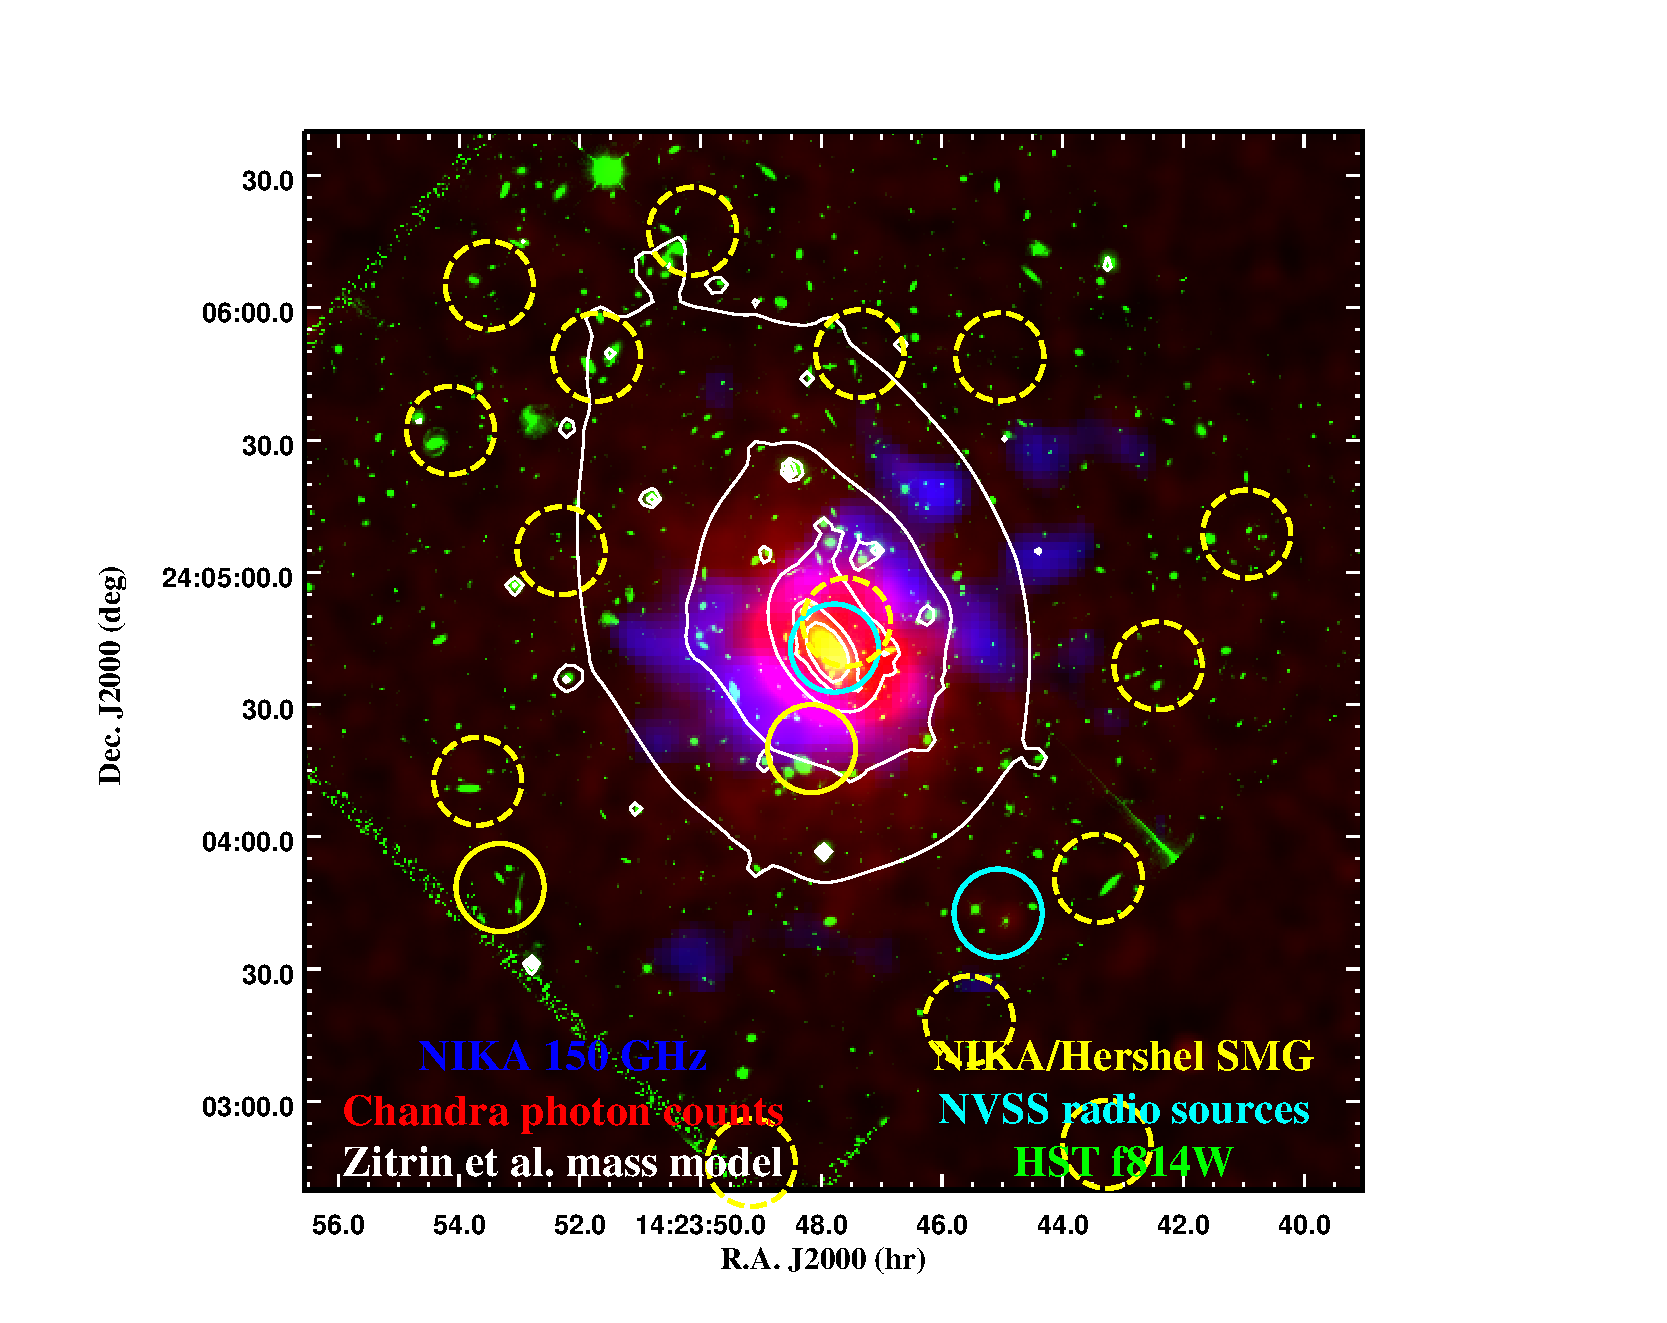
\includegraphics[trim=0cm 0cm 0cm 0cm, clip=true, width=0.99\textwidth]{Figure/MACSJ1424_multicolor.png}
\caption{Multi-wavelength dataset of \mbox{MACS~J1423.8+2404}. The origin of the data is given on top of each map. The maps have been smoothed and their range adapted for visualization purposes. The 10 arcsec radius circles give the point sources locations, in black/white for infrared sources and magenta for radio sources.}
\label{fig:MACSJ1424_mutiw2}
\end{figure*}

%---------- The multi-wavelenght picture
\begin{figure}[h]
\centering
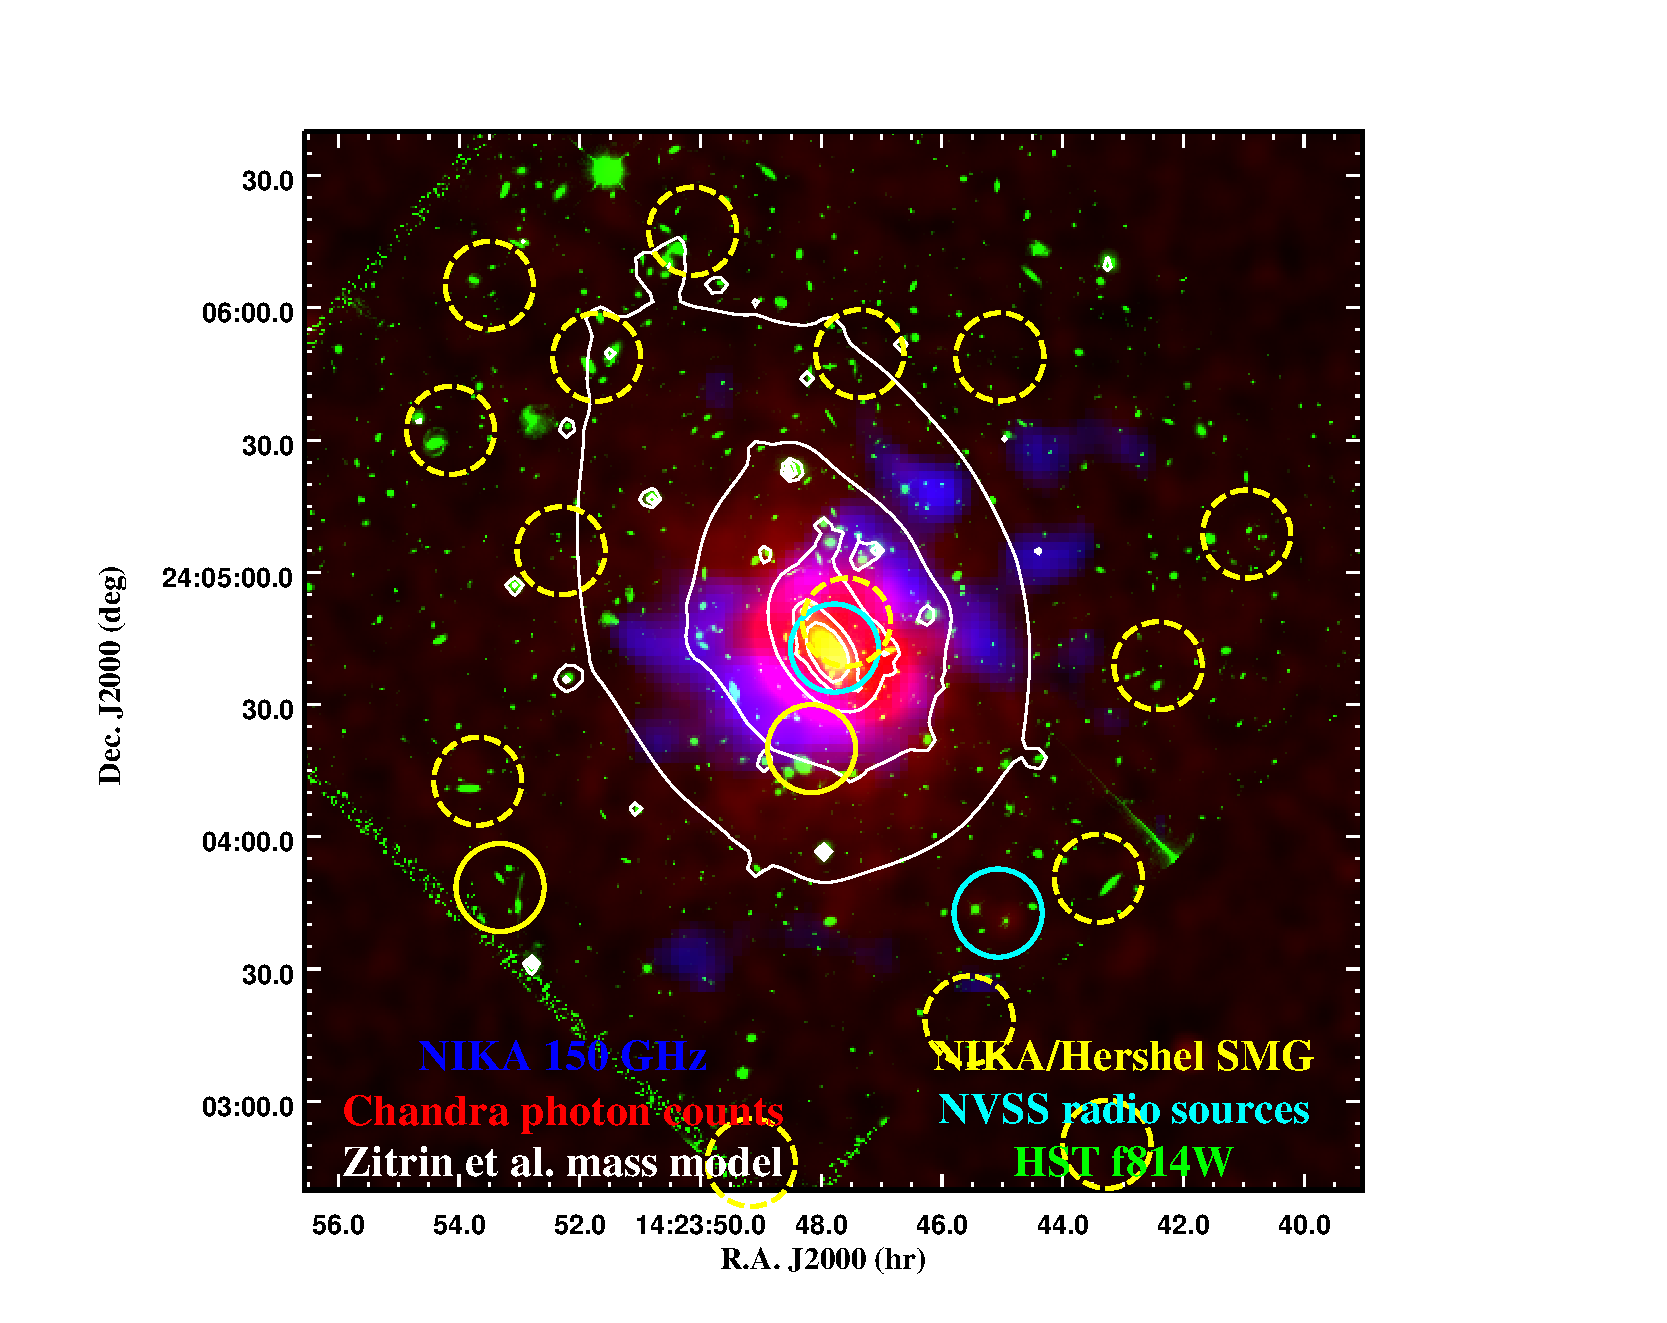
\includegraphics[trim=1cm 0cm 5cm 2cm, clip=true, width=0.45\textwidth]{Figure/MACSJ1424_multicolor.pdf}
\caption{Composite multi-wavelength image of \mbox{MACS~J1423.8+2404}. {\bf Blue image}: NIKA 150~GHz map showing the tSZ signal. {\bf Red image}: Chandra photon counts (ObsID04195) tracing the electronic density. {\bf White contours}: surface mass distribution model obtained by \cite{zitrin2011} in a linear scale. {\bf Yellow circles}: (sub-)millimeter sources candidate locations obtained using the NIKA 260~GHz map (solid line) and identified using Herschel (dashed-line). {\bf Cyan circle}: location of the radio point sources present in the field as obtained from VLA \citep{laroque2003}. {\bf Green image}: Hubble Space Telescope image using the F814W filter obtained by the CLASH  program \citep{postman2012} showing the location of optical galaxies.}
\label{fig:MACSJ1424_mutiw}
\end{figure}
We present in Fig.~\ref{fig:MACSJ1424_mutiw} a multi-wavelength image of \mbox{MACS~J1423.8+2404}. According to the X-ray literature, the cluster is a cool-core \citep[e.g.][]{kartaltepe2008} with a very low central temperature ($\sim 2$ keV) and a peak at $\sim 7$ keV at about 300 kpc away form the center \citep{morandi2010}. The Chandra map shows a relaxed morphology with a very peaked core and no significant substructure \citep{guennou2014}. The cluster is slightly elongated with the main axis oriented about 45 degrees clockwise with respect to the R.A. axis. The surface density mass models derived by \cite{limousin2010} and \cite{zitrin2011} agree with \mbox{MACS~J1424.8+2404} being elliptical and relaxed. \cite{limousin2010} report a mass within the inner 65 arcsec of $M(<65 \ {\rm arcsec}) = 4.3 \pm 0.6 \times 10^{14} \ {\rm M}_{\odot}$ which confirms that \mbox{MACS~J1423.8+2404} is indeed a massive system. The HST image is dominated by the central massive elliptical BCG (brightest cluster galaxy), which is coincident with the X-ray peak. The galaxy distribution does not show any particular group that would be the sign of a merging event. The BCG hosts a central AGN that is visible as a point source in radio observations \citep{laroque2003,condon1998,coble2007,bonamente2012}. This AGN is responsible for the presence of two cavities in the X-ray image \citep{hlavacek_larrondo2012}. Another radio source is located at about 1.5 arcmin south-west with respect to the X-ray peak. Background lensed and cluster members sub-millimeter galaxies are detected by Herschel. Two of those correspond to the excesses seen in the NIKA 260~GHz map. By using all the Herschel frequency bands, we find a total of 17 sub-millimeter sources. The NIKA 150~GHz detected tSZ signal is surrounding the cluster core. The hole seen in the tSZ signal is coincident with the BCG and results from the canceling of the tSZ by the radio and sub-millimeter signal.

%###############################################################################################
%##########################                POINT SOURCE CONTAMINATION             ##########################%###############################################################################################
\section{Radio and infrared point sources}\label{Radio_and_infrared_point_sources}
%========== Radio sources
\subsection{Radio point sources}
As discussed in Sect.~\ref{sec:Multi_wavelength_comparison}, the field around \mbox{MACS~J1423.8+2404} covered by NIKA is contaminated by two radio sources. The first one, hereafter RS1, is located within the central BCG, near the X-ray center. The second one, hereafter RS2, is located at about 1.5 arcmin towards the south-west. The flux of RS1 was measured at various radio wavelengths between 1.4 GHz and 30 GHz while the one of RS2 is only reported at 1.4 and 4.8 GHz. We list in Table~\ref{tab:Radio_ps} the fluxes measured for both sources.

To estimate the expected flux of each source in the NIKA bands, we model their SED by $F_{\nu} = F_{1 \ {\rm GHz}} \left(\frac{\nu}{1 \ {\rm GHz}}\right)^{\alpha_{\rm radio}}$. The fluxes reported in Table~\ref{tab:Radio_ps} are used to fit the amplitude of the SED, $F_{1 \ {\rm GHz}}$, and its slope, $\alpha_{\rm radio}$. The best-fit parameters are reported in Table~\ref{tab:Radio_ps} for both sources. We then simulate mock SED by sampling the parameters within their error bars and accounting for the covariance between them. Each mock SED is then integrated within the NIKA bandpasses to predict the expected flux at 150 and 260~GHz. The histogram of all the realizations is fitted by a gaussian function to give the expected fluxes and uncertainties, which are listed for both sources and both NIKA frequencies in Table~\ref{tab:Radio_ps2}.
\begin{table*}[h]
\caption{Location and flux (in mJy) of the radio sources observed in the $4 \times 4$ arcmin$^2$ field around \mbox{MACS~J1423.8+2404}.}
\begin{center}
\begin{tabular}{cccccc}
\hline
\hline
Source & Position & 1.4 GHz & 4.8 GHz & 28.5 GHz & 30 GHz \\
\hline
RS1 & 14:23:47.78 +24:04:42.8$^{(a)}$ & $8.0 \pm 1.1 ^{(b)}$ & $4.40 \pm 0.03 ^{(a)}$ & $1.49 \pm 0.12 ^{(c)}$ & $2.0 \pm 0.2 ^{(d)}$ \\  
RS2 & 14:23:45.07 +24:03:42.7$^{(a)}$ & $7.2 \pm 0.5 ^{(b)}$ & $2.72 \pm 0.03 ^{(a)}$ &  -- & --  \\  
\hline
\end{tabular}
\end{center}
{\small {\bf Notes.} $^{(a)}$ VLA, \cite{laroque2003}. $^{(b)}$ NVSS, \cite{condon1998}. $^{(c)}$ OVRO/BIMA, \cite{coble2007}. $^{(d)}$ SZA, \cite{bonamente2012}.}
\label{tab:Radio_ps}
\end{table*}

\begin{table*}[h]
\caption{Best-fit parameters and extrapolation of the fluxes (in mJy) in the NIKA bands of the radio sources in the $4 \times 4$ arcmin$^2$ field around \mbox{MACS~J1423.8+2404}. The degeneracy between the slope $\alpha_{\rm radio}$ and the amplitude $F_{1 \ {\rm GHz}}$ (given in mJy) has been accounted for to extrapolate the flux in the NIKA bands. See text for details.}
\begin{center}
\begin{tabular}{ccccccc}
\hline
\hline
Source & R.A. offset (arcsec) & Dec. offset (arcsec) & $F_{1 \ {\rm GHz}}$ & $\alpha_{\rm radio}$ & 150 GHz & 260 GHz \\
\hline
RS1 &      0.3 &      2.6 & $   10.39 \pm     0.30$ & $  -0.548 \pm    0.001$ & $    0.68 \pm     0.08$ & $    0.54 \pm     0.07$ \\
RS2 &     41.0 &    -57.3 & $    9.39 \pm     0.69$ & $  -0.790 \pm    0.003$ & $    0.18 \pm     0.04$ & $    0.13 \pm     0.03$ \\
\hline
\end{tabular}
\end{center}
\label{tab:Radio_ps2}
\end{table*}

%========== Submm sources
\subsection{Sub-millimeter point sources}
%---------- Herschel sources
We use the Herschel satellite catalog that contains the location and flux of the 17 sources found around \mbox{MACS~J1424.8+2404}. The 250 $\mu$m channel is the most complete one, with 15 sources, and we use it as a baseline to define the position of the sources and label. Thus, the corresponding sources in the other channels are identified on the basis of their positions. Due to the low resolution at 500 and 350 $\mu$m, a few sources are confused with their neighbors. Two sources peaking at high frequency are not present in the 250 $\mu$m catalog and we rely on the 100 $\mu$m channel for them. All the sources are not available for all the frequency bands in the catalog. Therefore, they are obtained by fitting the amplitude of a gaussian function on each map, at their reference location. The FWHM is fixed to the one of the respective Herschel channels. In addition, we fit also for a local background. In order to account for the confusion in the uncertainties, we fit randomly the same gaussian function at random positions, where the noise is homogeneous, and use the dispersion as the uncertainty. We check that the sources present in the catalog have compatible fluxes with respect to those we recover. The position and fluxes for all the sources are listed in Table~\ref{tab:IR_ps}.

%---------- Flux of the sources
Similarly, the fluxes of the sub-millimeter sources in the NIKA field are obtained by fitting the amplitude of a gaussian model. We use the NIKA FWHM at the expected sources positions as indicated by the Herschel data. We then correct them for the filtering induced by the data reduction, which is of the order of 15 percent for point sources. Uncertainties are obtained from the standard deviation of the amplitudes recovered using the gaussian fits performed on the Monte-Carlo noise map realizations. The fluxes obtained and their uncertainties are summarized in Table~\ref{tab:IR_ps} together with the Herschel data. For the SMG02 and SMG05 sources, the 150~GHz data is not included in the fit because of strong contamination by the local tSZ signal. By stacking the flux of all the sources, assuming that they are independent, we obtained an average flux of $2.84 \pm 0.79$ mJy at 260~GHz and $0.26 \pm 0.24$ mJy at 150~GHz, corresponding to a mean detection of 3.6 and 1.1 $\sigma$, respectively. 

\begin{table*}[h]
\caption{Positions and fluxes of the 17 sub-millimeter sources identified in the $4 \times 4$ arcmin$^2$ field around \mbox{MACS~J1423.8+2404}. All sources presenting negative best-fit fluxes are undetected and consistent with zero at 3 $\sigma$.}
\begin{center}
\begin{tabular}{ccccccccc}
\hline
\hline
Source & Position & 100 $\mu$m & 160 $\mu$m & 250 $\mu$m & 350 $\mu$m & 500 $\mu$m & 1.15 mm & 2.05 mm\\
\hline
%==================== Fluxes of the Herschel catalog
%SM01     & 14:23:52.31 +24:05:04.9 & $20.9 \pm 0.9$ & $35.3 \pm 3.2$ & $52.9 \pm 0.7$ & $31.5 \pm 0.6$ & $11.1 \pm 0.7$ & $ 2.1 \pm 3.3$ & $ 0.95 \pm 0.91$ \\  
%SM02     & 14:23:48.16 +24:04:20.0 & $12.0 \pm 0.9$ & $21.7 \pm 3.1$ & $33.7 \pm 0.7$ &            C05 &            C05 & $ 5.7 \pm 3.0$ & SZ \\  
%SM03     & 14:23:53.50 +24:06:05.1 & $10.6 \pm 0.9$ & $18.0 \pm 3.1$ & $36.5 \pm 0.8$ & $26.3 \pm 0.7$ &            C11 & $ 4.1 \pm 4.1$ & $ 1.08 \pm 1.08$ \\  
%SM04     & 14:23:42.42 +24:04:38.8 & $11.5 \pm 0.9$ & $17.6 \pm 3.0$ & $31.0 \pm 0.8$ & $19.6 \pm 0.7$ &           --   & $-1.6 \pm 3.3$ & $ 0.49 \pm 0.91$ \\  
%SM05     & 14:23:47.58 +24:04:48.7 & $ 5.9 \pm 0.9$ &           --   & $24.1 \pm 0.7$ &            C02 &            C02 & $ 3.7 \pm 2.9$ & SZ \\  
%SM06     & 14:23:53.32 +24:03:48.5 &          --    &           --   & $21.0 \pm 0.6$ & $16.0 \pm 0.6$ &           --   & $10.0 \pm 3.5$ & $ 1.88 \pm 0.96$ \\  
%SM07     & 14:23:45.04 +24:05:48.9 &          --    &           --   & $20.0 \pm 0.7$ & $15.2 \pm 0.8$ & $ 8.0 \pm 0.8$ & $ 1.2 \pm 3.6$ & $ 0.26 \pm 0.94$ \\  
%SM08     & 14:23:49.16 +24:02:46.1 &          --    &           --   & $19.5 \pm 0.7$ & $23.0 \pm 0.7$ & $ 9.0 \pm 0.8$ & $ 4.5 \pm 3.9$ & $ 0.69 \pm 1.05$ \\  
%SM09     & 14:23:43.27 +24:02:50.2 &          --    &           --   & $11.1 \pm 0.7$ &            C10 &            C10 & $ 2.2 \pm 4.3$ & $-0.87 \pm 1.11$ \\  
%SM10     & 14:23:44.55 +24:03:18.4 &          --    &           --   & $10.3 \pm 0.6$ &            C09 &            C09 & $ 1.5 \pm 3.5$ & $-0.54 \pm 0.94$ \\  
%SM11     & 14:23:54.14 +24:05:32.2 & $ 7.2 \pm 0.9$ &           --   & $ 9.4 \pm 0.6$ &          --    &            C03 & $ 0.7 \pm 4.0$ & $ 0.33 \pm 1.03$ \\  
%SM12     & 14:23:43.41 +24:03:50.6 & $ 5.4 \pm 0.9$ &           --   & $ 8.1 \pm 0.7$ &          --    &           --   & $ 2.2 \pm 3.5$ & $ 0.00 \pm 0.93$ \\  
%SM13     & 14:23:50.13 +24:06:17.4 & $11.9 \pm 0.9$ &           --   & $ 8.6 \pm 0.8$ &          --    &           --   & $-2.2 \pm 4.0$ & $ 0.99 \pm 1.05$ \\  
%SM14     & 14:23:47.36 +24:05:49.6 &          --    &           --   & $ 8.8 \pm 0.8$ &          --    &           --   & $ 0.6 \pm 3.3$ & $-0.58 \pm 0.89$ \\  
%SM15     & 14:23:40.95 +24:05:08.7 &          --    &           --   & $ 4.5 \pm 0.7$ &          --    & $ 9.5 \pm 0.7$ & $ 1.8 \pm 3.9$ & $ 0.20 \pm 0.99$ \\  
%SM16$^*$ & 14:23:53.69 +24:04:12.6 & $ 6.2 \pm 0.9$ &           --   &           --   &          --    &           --   & $ 6.5 \pm 3.4$ & $ 1.26 \pm 0.95$ \\  
%SM17$^*$ & 14:23:51.72 +24:05:48.8 & $ 4.9 \pm 0.9$ &           --   &           --   &          --    &           --   & $-0.6 \pm 3.8$ & $ 0.31 \pm 0.96$ \\
%====================
SMG01 & 14:23:52.31 +24:05:04.9 & $    20.8 \pm      1.0$ & $    35.2 \pm      3.3$ & $    52.3 \pm      7.7$ & $    28.9 \pm      7.0$ & $    11.3 \pm      9.2$ & $     1.4 \pm      3.1$ & $     0.9 \pm      0.9$ \\
SMG02 & 14:23:48.16 +24:04:20.0 & $    12.5 \pm      1.1$ & $    21.6 \pm      3.2$ & $    35.8 \pm     12.8$ & $    26.1 \pm      7.7$ & $    19.6 \pm      7.5$ & $     5.8 \pm      2.8$ & $^{**}$ \\
SMG03 & 14:23:53.50 +24:06:05.1 & $    10.8 \pm      1.1$ & $    17.5 \pm      2.9$ & $    34.7 \pm      8.5$ & $    26.4 \pm      8.0$ & $    10.3 \pm      8.6$ & $     6.1 \pm      3.6$ & $     0.7 \pm      1.0$ \\
SMG04 & 14:23:42.42 +24:04:38.8 & $    11.6 \pm      1.5$ & $    18.0 \pm      3.3$ & $    29.1 \pm      9.1$ & $    18.1 \pm     11.0$ & $     6.5 \pm      7.5$ & $     1.3 \pm      3.1$ & $     0.0 \pm      0.8$ \\
SMG05 & 14:23:47.58 +24:04:48.7 & $     6.4 \pm      1.6$ & $     9.1 \pm      2.7$ & $    25.6 \pm      8.4$ & $    23.0 \pm      7.6$ & $    19.9 \pm      8.8$ & $     3.8 \pm      2.8$ & $^{**}$ \\
SMG06 & 14:23:53.32 +24:03:48.5 & $     3.0 \pm      1.0$ & $     8.8 \pm      3.3$ & $    20.6 \pm     10.9$ & $    12.8 \pm      8.8$ & $   -11.0 \pm      7.7$ & $    11.5 \pm      3.2$ & $     1.4 \pm      0.9$ \\
SMG07 & 14:23:45.04 +24:05:48.9 & $     3.4 \pm      1.2$ & $    10.3 \pm      2.8$ & $    20.1 \pm      8.3$ & $    15.2 \pm      8.2$ & $     7.1 \pm      7.4$ & $     1.6 \pm      3.2$ & $     0.3 \pm      0.9$ \\
SMG08 & 14:23:49.16 +24:02:46.1 & $    -1.1 \pm      1.2$ & $     5.7 \pm      3.8$ & $    19.9 \pm      6.8$ & $    21.5 \pm      8.4$ & $     9.3 \pm      7.9$ & $     4.5 \pm      3.6$ & $     0.8 \pm      1.0$ \\
SMG09 & 14:23:43.27 +24:02:50.2 & $     2.5 \pm      1.4$ & $     5.5 \pm      3.2$ & $    12.6 \pm      8.1$ & $    20.2 \pm      9.5$ & $    22.3 \pm      8.6$ & $     1.9 \pm      4.0$ & $    -0.6 \pm      1.0$ \\
SMG10 & 14:23:44.55 +24:03:18.4 & $    -1.5 \pm      1.5$ & $     4.5 \pm      3.0$ & $    11.1 \pm      6.3$ & $    20.5 \pm      7.6$ & $    22.0 \pm      8.6$ & $     3.0 \pm      3.3$ & $    -0.7 \pm      0.9$ \\
SMG11 & 14:23:54.14 +24:05:32.2 & $     7.1 \pm      1.3$ & $    11.1 \pm      2.8$ & $    11.0 \pm      6.9$ & $    26.1 \pm      8.7$ & $     9.9 \pm      8.1$ & $    -0.5 \pm      3.5$ & $     0.3 \pm      1.0$ \\
SMG12 & 14:23:43.41 +24:03:50.6 & $     5.4 \pm      1.1$ & $     9.3 \pm      3.8$ & $     7.3 \pm     10.0$ & $   -10.4 \pm      9.9$ & $    -8.1 \pm      8.3$ & $     1.8 \pm      3.2$ & $    -0.1 \pm      0.9$ \\
SMG13 & 14:23:50.13 +24:06:17.4 & $    11.7 \pm      1.3$ & $     8.7 \pm      3.7$ & $     6.4 \pm      6.7$ & $   -11.8 \pm      9.5$ & $   -13.8 \pm      7.7$ & $    -2.0 \pm      3.6$ & $     0.9 \pm      1.0$ \\
SMG14 & 14:23:47.36 +24:05:49.6 & $     4.0 \pm      1.2$ & $     5.6 \pm      3.2$ & $     7.9 \pm     13.9$ & $    15.8 \pm      8.9$ & $     6.1 \pm      9.1$ & $     0.7 \pm      3.1$ & $    -0.7 \pm      0.8$ \\
SMG15 & 14:23:40.95 +24:05:08.7 & $     2.5 \pm      1.2$ & $     3.2 \pm      3.1$ & $     6.6 \pm      6.3$ & $     9.5 \pm      9.0$ & $     8.4 \pm      7.3$ & $    -0.5 \pm      3.4$ & $     0.0 \pm      0.9$ \\
SMG16$^*$ & 14:23:53.69 +24:04:12.6 & $     6.2 \pm      1.2$ & $     7.2 \pm      3.3$ & $    18.0 \pm      6.9$ & $   -10.9 \pm      9.3$ & $   -11.2 \pm      9.4$ & $     7.1 \pm      3.1$ & $     0.8 \pm      0.9$ \\
SMG17$^*$ & 14:23:51.72 +24:05:48.8 & $     4.7 \pm      1.2$ & $     3.7 \pm      3.4$ & $   -14.6 \pm      6.6$ & $    26.1 \pm      9.1$ & $     8.8 \pm      7.7$ & $    -1.1 \pm      3.3$ & $     0.1 \pm      0.9$ \\
\hline
\end{tabular}
\end{center}
{\small {\bf Notes.} $^*$ Sources for which the position is estimated based on the 100 $\mu$m PACS channel. $^{**}$ Fluxes which are not available due to the tSZ contamination.}
\label{tab:IR_ps}
\end{table*}

%---------- Modeling and fit of the SED
Only two sources are directly detected in the NIKA maps. In order to better constrain the fluxes within the NIKA bands, we model the SED by a modified black-body spectrum, $F_{\nu} = A_0 \left(\frac{\nu}{\nu_0}\right)^{\beta_{\rm dust}} B_{\nu}(T_{\rm dust})$. The parameter $A_0$ is a normalization, $\nu_0$ a reference frequency, $\beta_{\rm dust}$ the dust spectral index and $T_{\rm dust}$ the dust temperature. We notice a flux excess at 100 $\mu$m for most of the sources with respect to the best-fit SED derived from all the other channels, which we attribute to an extra dust component emission at higher frequency. We therefore exclude this frequency for constraining the SED in the following. 

We perform a Markov Chains Monte Carlo (MCMC) analysis to fit simultaneously for $\beta_{\rm dust}$ and $T_{\rm dust}$. This allows us to sample the corresponding parameter space and automatically marginalize over $A_0$, which is highly degenerated with the two other parameters. The Metropolis-Hasting algorithm is used to sample the parameter space. Each model tested against the data is defined by a value of $\beta_{\rm dust}$ and $T_{\rm dust}$ and the normalization is linearly adjusted to the data. For NIKA, color corrections are expected to be negligible with respect to the calibration and statistical uncertainties ($\sim 1-2$\%). In the case of Herschel, we apply the color corrections given in \cite{poglitsch2010} for PACS and those available at \url{http://herschel.esac.esa.int/Docs/SPIRE/html/spire_om.html\#x1-830005.2.6} for SPIRE. These coefficients are interpolated for each model using the values of $\beta_{\rm dust}$ and $T_{\rm dust}$, and provide a small correction to the Herschel fluxes ($\sim 5-10$\%). We finally obtain a set of models distributed with respect to the posterior likelihood. Each of the model SED spectra is integrated within the NIKA bandpasses and the distribution of fluxes gives the expected value and its uncertainty. The results are summarized in Table~\ref{tab:IR_ps2}.
\begin{table*}[h]
\caption{Location, and flux extrapolated to the NIKA channels for the 17 sub-millimeter sources identified in the $4 \times 4$ arcmin$^2$ field around \mbox{MACS~J1423.8+2404}.}
\begin{center}
\begin{tabular}{ccccccc}
\hline
\hline
Source &  R.A. offset & Dec. offset & 1.15 mm & 2.05 mm\\
\hline
SMG01 &    -61.8 &     24.9 & $    1.68 \pm     0.74$ & $    0.33 \pm     0.22$ \\
SMG02 &     -5.0 &    -20.0 & $    2.67 \pm     1.26$ & $    0.76 \pm     0.52$ \\
SMG03 &    -78.1 &     85.1 & $    1.98 \pm     0.99$ & $    0.45 \pm     0.31$ \\
SMG04 &     73.7 &     -1.2 & $    0.75 \pm     0.57$ & $    0.16 \pm     0.14$ \\
SMG05 &      3.0 &      8.7 & $    2.50 \pm     1.16$ & $    0.58 \pm     0.37$ \\
SMG06 &    -75.5 &    -51.5 & $    0.06 \pm     0.25$ & $    0.01 \pm     0.07$ \\
SMG07 &     37.8 &     68.9 & $    0.76 \pm     0.69$ & $    0.12 \pm     0.17$ \\
SMG08 &    -18.6 &   -113.9 & $    1.94 \pm     1.21$ & $    0.47 \pm     0.35$ \\
SMG09 &     62.1 &   -109.8 & $    2.23 \pm     1.36$ & $    0.44 \pm     0.35$ \\
SMG10 &     44.5 &    -81.6 & $    2.44 \pm     1.29$ & $    0.44 \pm     0.34$ \\
SMG11 &    -86.8 &     52.2 & $    0.63 \pm     0.76$ & $    0.14 \pm     0.18$ \\
SMG12 &     60.1 &    -49.4 & $    0.02 \pm     0.04$ & $    0.01 \pm     0.01$ \\
SMG13 &    -31.9 &     97.4 & $    0.03 \pm     0.04$ & $    0.00 \pm     0.01$ \\
SMG14 &      6.1 &     69.6 & $    0.32 \pm     0.59$ & $    0.05 \pm     0.11$ \\
SMG15 &     93.8 &     28.7 & $    0.03 \pm     0.19$ & $    0.04 \pm     0.12$ \\
SMG16$^*$ &    -80.6 &    -27.4 & $    0.02 \pm     0.05$ & $    0.00 \pm     0.01$ \\
SMG17$^*$ &    -53.6 &     68.8 & $    0.05 \pm     0.27$ & $    0.01 \pm     0.06$ \\
\hline
\end{tabular}
\end{center}
{\small {\bf Notes.} $^*$ Sources for which the position is estimated based on the 100 $\mu$m PACS channel.}
\label{tab:IR_ps2}
\end{table*}

%###############################################################################################
%##########################                SURFACE BRIGHTNESS PROFILE             ##########################%###############################################################################################
\section{Surface brightness profile}\label{sec:surface_brightness_profiles_comparison}
%---------- Method
Using the maps of Fig.~\ref{fig:flux_map} we compute the flux density profiles shown in Fig.~\ref{fig:flux_profiles} by averaging the signal within radial bins around the X-ray center. The error bars are computed by using the noise realizations described in Sect.~\ref{sec:Raw_NIKA_observations}. A flux density profile is computed for each noise realization and the standard deviation of all the realizations per radial bin provide the error bars associated to the profiles. This allows us to account for pixel--pixel noise correlation. We also compute the profile expected from the point sources for each NIKA band. This is done by simulating the corresponding maps using the point source fluxes and positions given in Tables~\ref{tab:Radio_ps} and~\ref{tab:IR_ps}. The profile is then calculated as for the NIKA maps and the error is given by the dispersion of Monte Carlo realizations of the point source maps by randomly varying the fluxes within their gaussian errors. We also add quadratically the NIKA calibration uncertainty to the error.

%---------- 150GHz
Fig.~\ref{fig:flux_profiles} shows that the 150~GHz profile decreases smoothly towards the center except in the inner 15 arcsec, were it rises. This is consistent with the positive signal expected from the point-like sources, dominated by the radio and the sub-millimeter ones in the cluster core. The cluster is detected, at the profile level, up to 60 arcsec radius. 

%---------- 260GHz
We notice that the sub-millimeter sources shown in Fig.~\ref{fig:MACSJ1424_mutiw} are located in two distinct regions. Two of them are within 30 arcsec from the X-ray peak, where we expect the tSZ contribution to be the strongest, while the others are concentrated in a ring of 70 arcsec inner radius and 130 arcsec outer radius. No source is seen around 50 arcsec from the cluster center. Despite the large error bars at 260~GHz, we see an excess near the center which we attribute to the sum of tSZ and sub-millimeter sources (from which one of them is detected with NIKA at the map level). A deep is seen around 1 arcmin, as expected form the source distribution, and another excess is seen around 100 arcsec from the center, attributed again to the Herschel sources. The NIKA 260~GHz profile is consistent with the one expected from point sources.
\begin{figure*}[h]
\centering
\includegraphics[height=6.4cm]{Figure/MACSJ1424_profile2mm_plus_ps.pdf}
\includegraphics[height=6.4cm]{Figure/MACSJ1424_profile1mm_plus_ps.pdf}
\caption{Profiles at 150~GHz (left) and 260~GHz (right), in units of surface brightness, of the raw map (black dots) and the contribution expected from radio and sub-millimeter point sources (red solid line). The red dashed envelope gives the 68\% confidence interval on the point sources profile.}
\label{fig:flux_profiles}
\end{figure*}

%###############################################################################################
%##########################                 PRESSURE RECONSTRUCTION                ##########################%###############################################################################################
\section{Radial pressure reconstruction}\label{sec:Radial_pressure_reconstruction}
%========== Xray
\subsection{XMM-Newton and Chandra X-ray data}
%++++++++++  Data prep.
\subsubsection{Data preparation}
MACSJ1423 cluster was observed by the Chandra Advanced CCD Imaging Spectrometer (ACIS) for \SI{115}{\kilo\second} (obs-ID $4195$) and by the XMM European Photon Imaging Camera (EPIC) for $\SI{109}{\kilo\second}$ in total (obs-IDs $720700301$ and $720700401$). XMM datasets were re-processed, applying the latest calibration files, using the Science Analysis System (SAS) version $14.0.0$ and calibrations files as available on May $2015$. Chandra datasets were re-processed using the Chandra Interactive Analysis of Observation (CIAO) software suite version $4.7$ and calibration database version $4.6.5$. To reduce contamination from the stationary flux of high energetic particles we applied the Very Faint mode\footnote{cxc.cfa.harvard.edu/cal/Acis/Cal\_prods/vfbkgrnd} filtering to Chandra datasets and for XMM we rejected events which keyword PATTERN (see, e.g., \citealt{pratt2007}) is $> 4$( for MOS$1,2$) and $>13$( for PN). 

Chandra and XMM datasets were analyzed using the very same technique so unless otherwise stated the procedures described in the following were applied to both datasets. To remove flare contamination we followed the procedures described in \cite{pratt2007} and in the Chandra COOKBOOK\footnote{cxc.harvard.edu/contrib/maxim/acisbg/COOKBOOK} for XMM and Chandra datasets, respectively, rejecting time intervals where the count rate exceeds $3\sigma$ the mean value. After the cleaning procedure we found no flare contamination in the Chandra dataset, and a useful exposure time of $\SI{122}{\kilo\second}$ for MOS$1$+MOS$2$ and $\SI{41}{\kilo\second}$ for PN.
To identify point sources we ran a wavelet detection algorithm with a threshold of $5\sigma$ on exposure corrected images in the $[0.3-2]\si{\kilo\electronvolt}$ and in $[0.7-7]\si{\kilo\electronvolt}$ bands for the Chandra and XMM datasets, respectively. The list of sources identified in both datasets were merged, inspected by eye and used as a mask to remove point source contributions from the analysis. 

%++++++++++  Vignetting correction
\subsubsection{Vignetting correction}
To correct for vignetting we followed the procedure described in \cite{arnaud2001}, computing for each photon a weight defined as the ratio of the effective area at the aimpoint and at  the photon position. Using these quantities we can perform imaging and spectroscopic analysis as if the detector had a flat response equal to that at the aimpoint. The weights were computed using the \verb?evigweight? routine for XMM, while for Chandra we used the procedure described in Bartalucci et al (in preparation). For each photon we also computed the effective exposure time, producing exposure maps that take into account bad pixels and columns. All the response files for weights and spectroscopic analysis were computed using the appropriate CIAO, \verb?mkarf? and \verb?mkacisrmf?, and SAS, \verb?arfgen? and \verb?rmfgen?, tools.

%++++++++++  Background subtraction
\subsubsection{Background subtraction}
The X-ray background is due to a diffuse sky emission and an instrumental component caused by the interaction of stationary high energetic particles with telescope instruments. To estimate the latter component we used datasets tailored to isolate this component, namely CLOSED (see \citealt{pratt2009}) and STOWED$^2$ for XMM and Chandra, respectively. To match the observation these datasets are skycasted and normalized in the $[10-12],[12-14]\si{\kilo\electronvolt}$ and in the $[9.5-10.6]\si{\kilo\electronvolt}$ band for MOS$1,2$-PN and ACIS, respectively. For Chandra we chose background datasets from period D, since the observation was performed during $2003$, as discussed in the COOKBOOK$^2$. We computed the weights for the instrumental background datasets applying the same point source masking and filtering procedures as for the observation datasets. We then subtracted from the surface brightness and temperature profiles the instrumental background evaluated using these datasets.

The residual background component is composed of a thermal Galactic emission \citep{snowden1995} and the blending of unresolved distant point sources, known as the cosmic X-ray background \citep{giacconi2001}. For the surface brightness profile analysis we determine a region free from cluster emission and subtract the residual mean background count rate. For the spectroscopic analysis we extracted the spectrum from the source free region and fitted it, through maximum likelihood estimation, with a multi component model, composed by two absorbed MEKAL and an absorbed power law (for details on the model used see \citealt{pratt2009}). The X-ray spectra in this work were extracted in the $[0.7-10]\si{\kilo\electronvolt}$ and in the $[0.3-10]\si{\kilo\electronvolt}$ band for Chandra and XMM datasets, respectively. When performing further spectroscopic analysis we added the background model as a fixed component whose amplitude is scaled by the ratio of the region of interest and background area.

%++++++++++  Pressure profile estimation
\subsubsection{Pressure profile estimation}
To compute the X-ray pressure profile we need to determine temperature and density profiles. 

The latter is computed by de-convolving and de-projecting the surface brightness profile using inversion with regularization as described in \cite{croston2006}. We extracted the surface brightness profile from concentric annuli centred on the X-ray peak, $RA$=$215.95$,$DEC$=$24.078$, in the $[0.3-2.5]\si{\kilo\electronvolt}$ and $[0.7-2.5]\si{\kilo\electronvolt}$ band from the $3$ combined EPIC and ACIS cameras, respectively. The profiles after background subtraction were re-binned by a logarithmic binning factor of $1.05$ to have a $3\sigma$ significance for each bin, and were PSF deconvolved using the analytical model of \cite{ghizzardi2001} for XMM. For Chandra we assume that the PSF is negligible with respect to 
the widths of the bins. 

The de-convolved and de-projected surface brightness profile were converted to a density profile using a conversion factor determined from the projected temperature profile. To determine this profile we extracted spectra from concentric annuli centred on the X-ray peak, the width of each annulus being defined to have a signal to noise ratio of $30$ after  background subtraction.  We measured the temperature in each bin by fitting the spectrum with an absorbed MEKAL model, where the absorption is fixed to $N_{H}=\SI{2.2e20}{\centi\meter}^{-3}$ \citep{kalberla2005}, redshift to $z=0.545$, plus the scaled sky background component discussed above. To interpolate the temperature profile for each surface brightness bin we fit to the observed temperature profile with the parametric model described in \cite{vikhlinin2006}. 

To de-project the temperature profile we measured the spectroscopic-like temperature \citep{mazzotta2004} using the weighting scheme implemented in \cite{vikh_multit}, where the observed temperature profile is modelled as the weighted sum of concentric plasma shells each at a different temperature. As for the density profiles, we take in account the PSF effects for XMM. Pressure profiles are then computed as the product of the de-projected temperature and density profiles. As we can see from left image of Figure 8, where we show the de-projected temperature profiles of XMM and Chandra, in dark and light blue, respectively, the two profiles are in good agreement over the entire radial range. The profiles are in good agreement also in the shape, both showing a peak of the temperature at the same radius $\sim \SI{180}{\kilo\parsec}$, even though the Chandra profile is systematically lower $\sim \SI{1}{\kilo\electronvolt}$, contrary to what is generally found (e.g. \citealt{mahdavi2013} or \citealt{martino2014}). 

%========== Modeling
\subsection{Modeling}\label{sec:modeling}
%---------- What we do
We model the cluster ICM using the same approach adopted for another NIKA cluster, described in details in \cite{adam2014}. As seen in Sect.~\ref{sec:Multi_wavelength_comparison} and emphasized by \cite{morandi2010}, \mbox{MACS~J1423.8+2404} is elliptical. Nevertheless, we assume spherical symmetry because this work does not focus on its geometry, but on the impact of the presence of point sources on the pressure profile reconstruction. Moreover, the significance of the NIKA 150~GHz tSZ map is not sufficient to constrain this asymmetry. We summarize here the procedure adopted to recover the cluster radial physical properties.

%---------- tSZ
The tSZ effect \citep{sunyaev1972,sunyaev1980} results in a distortion of the CMB black-body spectrum relative to the primary CMB intensity, $I_0$, \citep[e.g.][]{birkinshaw1999}
\begin{equation}
	\frac{\Delta I_{tSZ}}{I_0} = y \ f(\nu, T_e).
\label{eq:deltaI}
\end{equation}
The function $f(\nu, T_e)$ gives the characteristic frequency dependence of the spectrum. The small dependance on the electronic temperature, $T_e$, arises from relativistic corrections for which we use the results of \cite{itoh1998}. The Compton parameter, $y$, gives the amplitude of the distortion and is related to the line of sight integral of the electronic pressure, $P_e$, as 
\begin{equation}
	y = \frac{\sigma_{\mathrm{T}}}{m_{e} c^2} \int P_{e} dl.
	\label{eq:y_compton}
   \end{equation}
The parameter $\sigma_{\mathrm{T}}$ is the Thomson cross section, $m_{e}$ is the electron rest mass, and $c$ the speed of light. The total integrated tSZ flux, $Y$, is then given by the aperture photometry performed on the Compton parameter map.

%---------- Model
The cluster electronic pressure radial distribution is modeled by a gNFW profile \citep{nagai2007}, described by
\begin{equation}
	P_e(r) = \frac{P_0}{\left(\frac{r}{r_p}\right)^c \left(1+\left(\frac{r}{r_p}\right)^a\right)^{\frac{b-c}{a}}}.
\label{eq:gNFW}
\end{equation}
The parameter $P_0$ is a normalization constant; $r_p$ is a characteristic radius; and $a$, $b$, and $c$ set the slopes at intermediate, large, and small radii, respectively. This model is chosen to allow the description of the profile at all scales. The electronic density is modeled by a \emph{Simplified Vikhlinin Model} \citep{vikhlinin2006},
\begin{equation}
	n_e(r) = n_{e0} \left[1+\left(\frac{r}{r_c}\right)^2 \right]^{-3 \beta /2} \left[ 1+\left(\frac{r}{r_s}\right)^{\gamma} \right]^{-\epsilon/2 \gamma}.
\label{eq:SVM}
\end{equation}
The parameter $n_{e0}$ is the central density, $r_c$ is the core radius and $\beta$ is related to the slope of the profile. The second term allows the description of the steepening of the profile at large scales. The parameter $\epsilon$ gives the change in the slope, $r_s$ the radius at which the transition occurs, and $\gamma$ the width of the transition. In the following, we set $\gamma = 3$ since it provides a good fit to all clusters considered in the analysis of \cite{vikhlinin2006}.

With the pressure and the density in hand, we compute the temperature profile assuming the ideal gas law, $k_B T_e(r) = \frac{P_e(r)}{n_e(r)}$, and the entropy profile as $K(r) =  \frac{P_e(r)}{n_e(r)^{5/3}}$ following \cite{voit2005}. The total mass, assuming hydrostatic equilibrium, enclosed within $r$ is then given by $M_{\rm HSE}(r) = -\frac{r^2}{\mu_{gas} m_p n_e(r) G} \frac{dP_e(r)}{dr}$.

%---------- Fit
The parameter space is sampled using the Markov Chain Monte Carlo approach detailed in \cite{adam2014}. We jointly fit the 150~GHz NIKA tSZ map, the electronic density profile computed from the deprojection of the X-ray data. In addition, we add a constraint on the total tSZ flux of the cluster using the Planck Compton parameter map \citep{planck2015XXII}. The tSZ models are convolved with the effective transfer function of the observations, including the beam smoothing and the large scale filtering cutoff due to the removal of the atmospheric noise. The cluster \mbox{MACS~J1423.8+2404} is not present in the Planck catalogue of tSZ sources \citep{planck2015XXVII}, but we obtain an upper bound on its flux by integrating the Compton parameter map \citep{planck2015XXII} using aperture photometry. The error on the flux is computed by performing the same measurement randomly around the cluster, where the noise is homogeneous. The flux is measured to be $Y_{\rm tot}^{\rm Planck} = \left(0.40 \pm 0.66\right) \times 10^{-3}$ arcmin$^2$. During the MCMC sampling, we also marginalize over nuisance parameters such as the zero level of the NIKA map, the calibration uncertainty, or the central point source flux and position when included in the fit. See \cite{adam2014} for more details.

%========== Results
\subsection{Results}
The cluster \mbox{MACS~J1423.8+2404} is known to be a typical cool-core \citep[e.g.][]{kartaltepe2008}. Therefore, we use as a baseline the pressure profile slopes found for such clusters by \cite{arnaud2010}: $\left(a,b,c\right) = \left(1.2223, 5.4905, 0.7736\right)$. The angular resolution of XMM-Newton and NIKA are similar and the complementarity of the two experiments will be used in the future tSZ dedicated NIKA2 large program. This is why, in the present work, XMM-Newton is used as a reference and we cross-check our results with Chandra data.

%++++++++++ Test of the point sources
\subsubsection{Impact of the point sources}
%---------- How to test point impact of sources
The impact of the point source contamination on the reconstructed pressure profile is tested by considering three different cases: 
\begin{enumerate}
\item The presence of point sources is ignored and we fit the parameters $P_0$ and $r_p$, keeping the slope parameters fixed to their baseline values. This case is referred as model 1 (M1).
\item The point sources are subtracted assuming the fluxes of Table \ref{tab:IR_ps2} and we repeat the fit of model M1. This case is referred as model 2 (M2).
\item The point sources are subtracted assuming the fluxes of Table \ref{tab:IR_ps2}, but possible residuals of the central sources are also fitted. In this case, we also release the constraint on the inner and outer slope parameters, $c$ and $b$, which are also fitted. The intermediate slope parameter $a$ is held fixed because it is strongly degenerated with the characteristic radius $r_p$ and the outer slope $b$. This case is referred as model 3 (M3).
\end{enumerate}
The comparison of the output pressure profile of models M1 and M2 (see Fig.~\ref{fig:MACSJ1424_pressure_point_source}) allows a direct estimation of the impact of point sources. The use of model M3 is motivated by the large uncertainties on the point source fluxes as shown in Table \ref{tab:IR_ps2}. As discussed in Sect.~\ref{sec:surface_brightness_profiles_comparison} and shown on Fig.~\ref{fig:flux_profiles}, the sources that are in the outer region of the cluster do not contribute significantly to the radial flux density. However, this is not the case for the central sources, in particular for RS1 and SMG05. We expect a significant correlation between the flux of theses sources and the pressure profile parameters related to the cluster core, such as $P_0$, $r_p$ and $c$. Those related to the external regions of the profile are also affected, due to projection effects. Therefore, model M3 allows to test the constraint that can be obtained on the pressure profile at the cluster core in the presence of a contaminating central point source, when no strong prior on its flux is available, as it is the case here.

%---------- Results on the constrained profile
The pressure profile measured in the three cases is given in Fig.~\ref{fig:MACSJ1424_pressure_point_source}. Model M1 is lower than the two other at all scales, except above 1000 kpc where NIKA do not provide a direct constraint, due to the large scales filtering. This corresponds to the fact that point sources, and in particular those close to the core, compensate the overall flux amplitude of the cluster. Apart from its normalization factor, the shape of the pressure profile is similar for M1 and M2 as the constraint on the parameter $r_p$ is not significantly affected by the point sources subtraction. The effect of the source in the cluster core is then diluted in the parameter degeneracy over all the profile via $P_0$ and $r_p$. The results for M3 are close to those of M2 but error contours are larger because of the extra freedom available in the parameter space. This is particularly true in the inner region, where the error on the flux of the fitted point source propagates to the profile via the degeneracies between parameters. Therefore, the inner pressure distribution remains unconstrained unless the point sources is subtracted with sufficient accuracy. At large scales, around 800 kpc, the preferred model M3 is slightly above the M2 one. However, it is important to notice that the differences observed between models are not significant with respect to the uncertainties, which are dominated by the low exposure time spent with NIKA on this cluster.
\begin{figure}[h]
\centering
\includegraphics[width=0.49\textwidth]{Figure/ICM_pressure_profile_point_sources.pdf}
\caption{Constraint on the pressure profile of \mbox{MACS~J1423.8+2404} for the three models M1 (green), M2 (orange) and M3 (red). The solid lines gives the central profiles and the dashed line represent the 68\% confidence limits.}
\label{fig:MACSJ1424_pressure_point_source}
\end{figure}

%---------- Morphology
The best-fit model of M3 is subtracted from the NIKA 150~GHz map to search for possible deviations from the spherical relaxed morphology, as expected according to X-ray and lensing observations. Fig.~\ref{fig:MACSJ1424_MCMC_modeling} represents the raw, point sources subtracted, tSZ best-fit, and residual 150~GHz maps. After removing the point sources (fluxes in Table \ref{tab:IR_ps2}) and the best-fit of model M3, the cluster appears to be fairly compact with a small excess towards the south. However, the significance of the latter is less than 2 $\sigma$ and can be attributed to a poor subtraction of SMG05, whose position is very close on the map. The signal is on overall relatively spherical, as confirmed by the residual ({\it i.e.} the difference between the point source removed map and the best-fit tSZ spherical model), which is consistent with the noise. Deeper tSZ observations would be necessary in order to further constrain the cluster morphology, in particular in terms of ellipticity.
\begin{figure*}[h]
\centering
\includegraphics[width=0.49\textwidth]{Figure/MCMC_raw_map.pdf}
\includegraphics[width=0.49\textwidth]{Figure/MCMC_point_source_removed.pdf}
\includegraphics[width=0.49\textwidth]{Figure/MCMC_best_fit.pdf}
\includegraphics[width=0.49\textwidth]{Figure/MCMC_residual.pdf}
\caption{Comparison of the raw 150~GHz input NIKA map (top left), the same map after point sources subtraction (top right), the best-fit tSZ model (bottom left), and the final residual map. Contours are the same as in Fig.~\ref{fig:flux_map}, they give the significance in unit of $\sigma$, starting from $\pm 2 \ \sigma$. Uncertainties arising from the point sources and the model subtraction are ignored on these contours.}
\label{fig:MACSJ1424_MCMC_modeling}
\end{figure*}

%++++++++++ X vs SZ
\subsubsection{Comparison between tSZ and X-ray derived cluster thermodynamics}
%---------- Flux density profile
Fig.~\ref{fig:MACSJ1424_MCMC_pressure_profile} presents the best-fit and the uncertainties of model M3 on the projected flux density profile, and compares it with the NIKA data subtracted from the point sources based on Table \ref{tab:IR_ps2}. It is important to notice that the data points are correlated across the profile. We account for this in the MCMC analysis. The uncertainties increase significantly in the cluster core because the flux estimate (and associated error) of the central point source is included in the fit. The model is greater than zero at large scales because the zero level of the map (one of the nuisance parameters included in the fit), is positive.

%---------- Pressure profile
The right panel of Fig.~\ref{fig:MACSJ1424_MCMC_pressure_profile} shows the deprojected pressure profile of \mbox{MACS~J1423.8+2404} as derived from our MCMC analysis and from X-ray measurement only. While deep X-ray observations can only infer the pressure, the tSZ effect directly measures it. The comparison of the two, which are completely independent, is therefore an important cross check for both constraints. In the right panel of Fig.~\ref{fig:MACSJ1424_MCMC_pressure_profile}, the data points represent measurements obtained from XMM-Newton and Chandra, and the shaded area is the 68\% confidence limit given by model M2. The upper and lower dashed lines give respectively the upper and lower limits from all the tSZ based models M1, M2 and M3. The Chandra constraint is slightly more peaked than the XMM-Newton one. In turn, the latter is slightly more peaked than the tSZ one, but all of them are compatible within error bars. These results confirm that the point spread function deconvolution of the XMM-Newton data performs well and that the model extrapolation of the tSZ data accurately describes the pressure profile at the cluster center. At large radii, the Chandra measurement is not available due to a photon count rate lower than XMM-Newton making the two observations are complementary. The tSZ measured pressure profile decreases slightly slower than the X-ray one but this effect is not significant with respect to the uncertainties.
\begin{figure*}[h]
\centering
\includegraphics[height=6.3cm]{Figure/MACSJ1424_profile_ML.pdf}
\includegraphics[height=6.3cm]{Figure/ICM_pressure_profile_xray.pdf}
\caption{MCMC constraints on the pressure distribution in terms of projected and deprojected profiles. {\bf Left}: projected tSZ flux density profile for the point sources subtracted NIKA data (black dots) and for the M3 best-fit model (red solid line). Uncertainties at 68\% confidence limits are given by the red dashed lines. {\bf Right}: deprojected pressure profile. The Chandra (CXO for Chandra X-ray Observatory) and XMM-Newton measurements are given by the blue diamonds and the purple dots, respectively. The red shaded area provides the MCMC 68\% confidence limit from model M2, the central solid line corresponding to the best-fit model. The two dashed lines give the upper and lower limits allowed considering all three models M1, M2 and M3 (see Fig.~\ref{fig:MACSJ1424_pressure_point_source}).}
\label{fig:MACSJ1424_MCMC_pressure_profile}
\end{figure*}

%---------- Entropy and temperature
The constraints on temperature and entropy, directly related to the ones from the pressure and the density (see Sect.~\ref{sec:modeling}), are given in Fig.~\ref{fig:MACSJ1424_MCMC_tk_profile}. The red contours use the tSZ derived pressure and the XMM-Newton derived density, while the data points are X-ray only deprojected measurements based on spectroscopic data. Since both the temperature and the entropy are proportional to the pressure, this figure reproduces the comparison of the right panel of Fig.~\ref{fig:MACSJ1424_MCMC_pressure_profile} focussing on different thermodynamic quantities. The temperature profile is typical of a cool-core cluster with a core temperature of about 5 keV, and reaches about 10 keV at a radial distance of 200 kpc. The entropy is well described by a single power law up to the cluster core, confirming that \mbox{MACS~J1423.8+2404} is relaxed \citep{guennou2014}. At large scales, both XMM-Newton and tSZ derived constraints indicate a flattening of the profile.
\begin{figure*}[h]
\centering
\includegraphics[height=6.3cm]{Figure/ICM_temperature_profile.pdf}
\includegraphics[height=6.3cm]{Figure/ICM_entropy_profile.pdf}
\caption{Deprojected radial temperature profile (left) and radial entropy profile (right). The legend is the same as in Fig.~\ref{fig:MACSJ1424_MCMC_pressure_profile}.}
\label{fig:MACSJ1424_MCMC_tk_profile}
\end{figure*}

%---------- Mass
In addition to the cluster thermodynamics, the assumption of the hydrostatic equilibrium allows us to derive the mass of the cluster. We obtain $M_{500} = 6.9^{+6.5}_{-2.9}  \times 10^{14} {\rm M}_{\odot}$ for model M3. The total integrated Compton parameter is also constrained to be $Y_{\rm tot} = 0.85^{+0.61}_{-0.30} \times 10^{-3}$ arcmin$^2$, in agreement but slightly larger than the Planck value.

%---------- Discusion
Both XMM-Newton and Chandra results present error bars smaller than those derived from NIKA+Planck tSZ data. Nevertheless, we emphasize that both X-ray data sets are particularly exceptional for this cluster (about 30 hours of exposure time for both instruments), while the tSZ ones have been obtained with only 1.47 hours on target. Even in this situation, NIKA already provides essential informations that allow the reconstruction of the thermodynamical structure of the the cluster to reasonable accuracy when combined to X-ray.

%###############################################################################################
%##########################                DISCUSSION AND CONCLUSION                ##########################%###############################################################################################
\section{Conclusions and prospectives}\label{sec:conclusions}
%++++++++++ Prospectives
\subsection{Conclusions}
%---------- NIKA observations
The cluster of galaxies \mbox{MACS~J1423.8+2404} was observed at 150 and 260~GHz using the NIKA camera at the IRAM 30m telescope. The target is detected at 150~GHz in only 1.47 hours and the data show evidence for the presence of a contaminating central point source, as expected from radio observations. The 260~GHz NIKA band allows the identification of two sub-millimeter contaminant galaxies.

%---------- Multi-wavelenght observations
NIKA observations were combined to external datasets in multiple wavelengths to qualitatively assess the cluster morphology and the dynamical state of the gas. The object \mbox{MACS~J1423.8+2404} is a typical cool-core, which appears to be relaxed and elliptical. A total of 17 sub-millimeter sources were identified in the NIKA field using Herschel data, and two radio sources were known from external radio observations.

%--------- Sources
The fluxes of the two radio sources have been extrapolated to the NIKA bands by fitting a power law SED to external photometric measurements. The sub-millimeter sources were extrapolated to the NIKA bands by modeling their SED with a grey-body spectrum and fitting jointly the Hershel satellite and NIKA photometric data. This work shows the strong complementarity between the two instruments in terms of frequency coverage and angular resolution. The comparison of the flux density derived from NIKA data directly shows a good agreement with the expectation from the point sources extrapolated fluxes at the same frequencies. The contamination from point sources can, therefore, be estimated and subtracted from the tSZ map, if external data are available at complementary wavelengths.

%---------- Profile
The pressure profile of \mbox{MACS~J1423.8+2404} was then measured by modeling and fitting jointly the NIKA and Planck data. We have evaluated the impact of the point sources contamination on its reconstruction. We find that neglecting the sources leads to an overall underestimate of the profile, which is small compared to the error bars in the case of the available data, but that could become significant when deeper tSZ observations are available. Moreover, in the case of the presence of a point source at the cluster center with no strong priors on its flux, the inner pressure profile remains poorly constrained by the data. We used XMM-Newton and Chandra X-ray observations to derive the cluster thermodynamical radial distributions. The deprojected electronic density has been combined to the tSZ data, which provides a measurement of the pressure, to infer the temperature and the entropy profiles. The X-ray only (including spectroscopy) and the tSZ+X-ray (without spectroscopy) constraints are consistent within error bars, and confirm that \mbox{MACS~J1423.8+2404} is a relaxed cool-core cluster.

%++++++++++ Prospectives
\subsection{Prospect for NIKA2 observations}
%---------- Prospect for NIKA2
These observations and study are part of the NIKA tSZ pilot study aiming at characterizing the outcomes of the tSZ large program, which is in preparation for the future camera NIKA2. NIKA2 will be used to observe about 50 clusters at intermediate and high redshift ($z>0.5$) in order to study the pressure distribution in this class of objects. Clusters are crowded environments, therefore, in high angular resolution tSZ observations (like those of NIKA2) we expect the detection of a large number of point sources, as demonstrated in \cite{adam2013}, \cite{adam2014} and in the present work. These sources are a contaminant in the context of tSZ studies. We have shown here that their contribution can be estimated and accounted for in tSZ analysis if external data are available. Sub-millimeter point sources should not be a problem because they can be identified at 260~GHz and marginalized over at 150~GHz. They can even be masked without removing the information on the profile. Radio point sources can be more problematic. Unless they are as strong as the tSZ signal, they can only be identified using external data. They are generally correlated with the central BCG and will refrain NIKA2 to put any constraint on the cluster core pressure unless their SED is well measured at lower frequencies. If no external data are available, the removal of the contaminants will require the use of extra high angular resolution observations obtained with interferometers at similar frequencies, such as the IRAM NOrthern Extended Millimeter Array (NOEMA)\footnote{\url{http://iram-institute.org/EN/noema-project.php}}. Point sources around clusters are also interesting in themselves and the high complementarity between Herschel and NIKA could be used, for example, to search for distant lensed galaxies \citep[see for example][]{egami2010} or to study star formation at high redshift. This will be an extra outcome of the NIKA2 tSZ large program.

The present work has also shown how X-ray and tSZ data can be used to constrain the temperature and the entropy profiles of galaxy clusters independently from X-ray spectroscopy, using the density and pressure profiles. Moving to high redshift, X-ray spectroscopy, which is necessary to derive the electronic temperature from X-ray data, gets time expensive and high-quality X-ray mapping becomes challenging, due to the redshift dimming. In this context, the results obtained in this study show that we are able to constrain the ICM thermodynamics with a good accuracy by combining resolved NIKA tSZ observations and X-ray mapping. This will be particularly important for NIKA2 distant clusters, for which we will not benefit from deep enough X-ray observations, and where only a mean temperature can be obtained from X-ray data. In addition, X-ray constraints on the cluster thermodynamics directly depend on the energy calibration of the instrument, which is quite often a source of discrepancy between XMM-Newton and Chandra observations \citep[see for example the recent work of][]{schellenberger2015}. NIKA tSZ data provide a third independent measurement, independent from X-ray spectroscopy and related systematics, providing a cross check of the temperature measurement of clusters. This can help reducing the systematic effects affecting all these observations, which are essential for mass estimates when using clusters as a cosmological probe.

%###############################################################################################
%##########################                       ACKNOWLEDGEMENTS                        ##########################%###############################################################################################
\begin{acknowledgements}
We would like to thank the IRAM staff for their support during the campaign.
This work has been partially funded by the Foundation Nanoscience Grenoble, the ANR under the contracts "MKIDS" and "NIKA". 
This work has been partially supported by the LabEx FOCUS ANR-11-LABX-0013. 
This work has benefited from the support of the European Research Council Advanced Grant ORISTARS under the European Union's Seventh Framework Program (Grant Agreement no. 291294).
The NIKA dilution cryostat was designed and built at the Institut N\'eel. In particular, we acknowledge the crucial contribution of the Cryogenics Group and, in particular Gregory Garde, Henri Rodenas, Jean Paul Leggeri, and Philippe Camus. 
R. A. would like to thank the ENIGMASS French LabEx for funding this work. 
B. C. acknowledges support from the CNES post-doctoral fellowship program. 
E. P. acknowledges support from grant ANR-11-BS56-015. 
The mass model used in this paper was constructed by \cite{zitrin2011}, and obtained through the Hubble Space Telescope Archive, as a high-end science product of the CLASH program \citep{postman2012}.
\end{acknowledgements}

\bibliography{biblio_macsj1424}
\end{document}